\documentclass[main]{subfiles}

\begin{document}

The firmware of the MCU has 2 working modes, which can be selected at startup, 
with the supply voltage (figure \ref{FIG_FW_STARTUP_FC}):
\begin{itemize}
    \item Calibration Mode 
    \item Normal Mode
\end{itemize}

\begin{figure}[h]
    \centering
    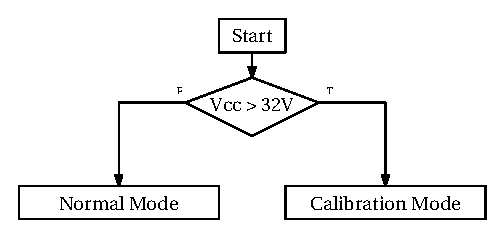
\includegraphics[width=0.8\linewidth]{img/fw_mode_sel_flowchart.eps} 
    \caption{Firmware startup mode selection}
    \label{FIG_FW_STARTUP_FC}
\end{figure}

If you power the device at $32 V$, it enters the calibration mode, it samples 
analog signals while the rotor spins, and performs calculations, without driving 
output signals.
After it has acquired enough samples, it saves calibration parameters inside its
non-volatile memory, and it stays idle until a power cycle is performed.

Powering the device at any voltage below $24 V$ makes it enter normal mode, it 
samples analog signals, it applies compensation with previously saved parameters,
calculates position and generates output signals.  

\end{document}